 \subsection{Høvsøre}
\begin{figure}[H]
	\begin{minipage}{0.33\linewidth}
		\centering \hspace{1.5cm}(a)
	\end{minipage}%
	\begin{minipage}{0.33\linewidth}
		\centering \hspace{1cm}(b)
	\end{minipage}%
	\begin{minipage}{0.33\linewidth}
		\centering \hspace{1cm}(c)
	\end{minipage}%
	\vspace{-3mm}
	\begin{center}
		\includegraphics[height=0.62\linewidth,page=37,trim={35mm 10mm 41mm 25mm},clip]{Imagenes/06/hov/9u}%
		\includegraphics[height=0.62\linewidth,page=37,trim={48mm 10mm 41mm 25mm},clip]{Imagenes/06/hov/9v}%
		\includegraphics[height=0.62\linewidth,page=37,trim={48mm 10mm 41mm 25mm},clip]{Imagenes/06/hov/9V}%
	\end{center}
	\caption{Comparación de la simulación (línea continua) con la simulación de Peña et. al. en el 2013 (línea punteada) y valores medidos para (a) componente $u$ de la velocidad del viento, (b) componente $v$ y (c) magnitud de la velocidad del viento. Los datos corresponden a promedios temporales entre las 12:00 y 15:00, y han sido rotados de tal forma que su dirección sea 0$^\circ$ a los 10m.}
	\label{fig:06_hov_pena}
\end{figure}

\begin{figure}[H]
	\centering
	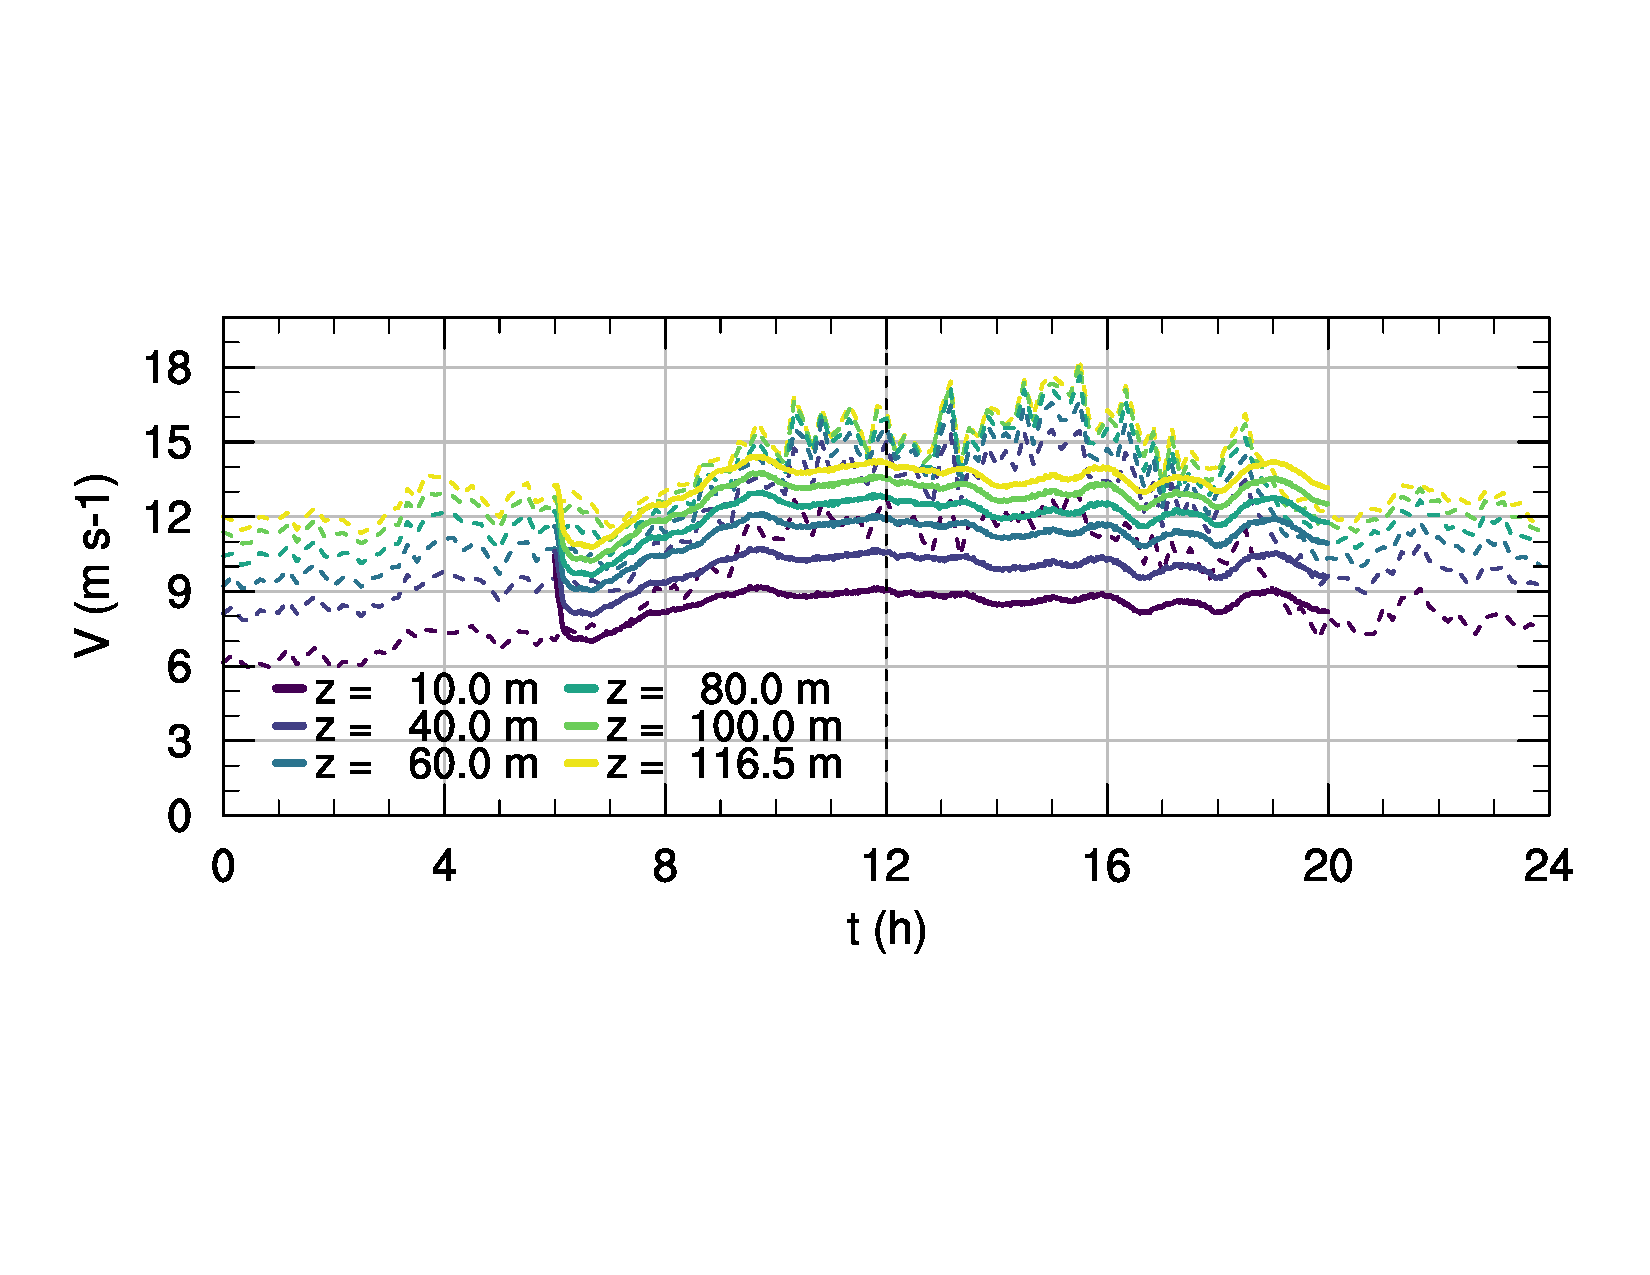
\includegraphics[width=0.5\linewidth,trim={9mm 63mm 10mm 55mm},clip]{Imagenes/06/hov/ts_v}%
	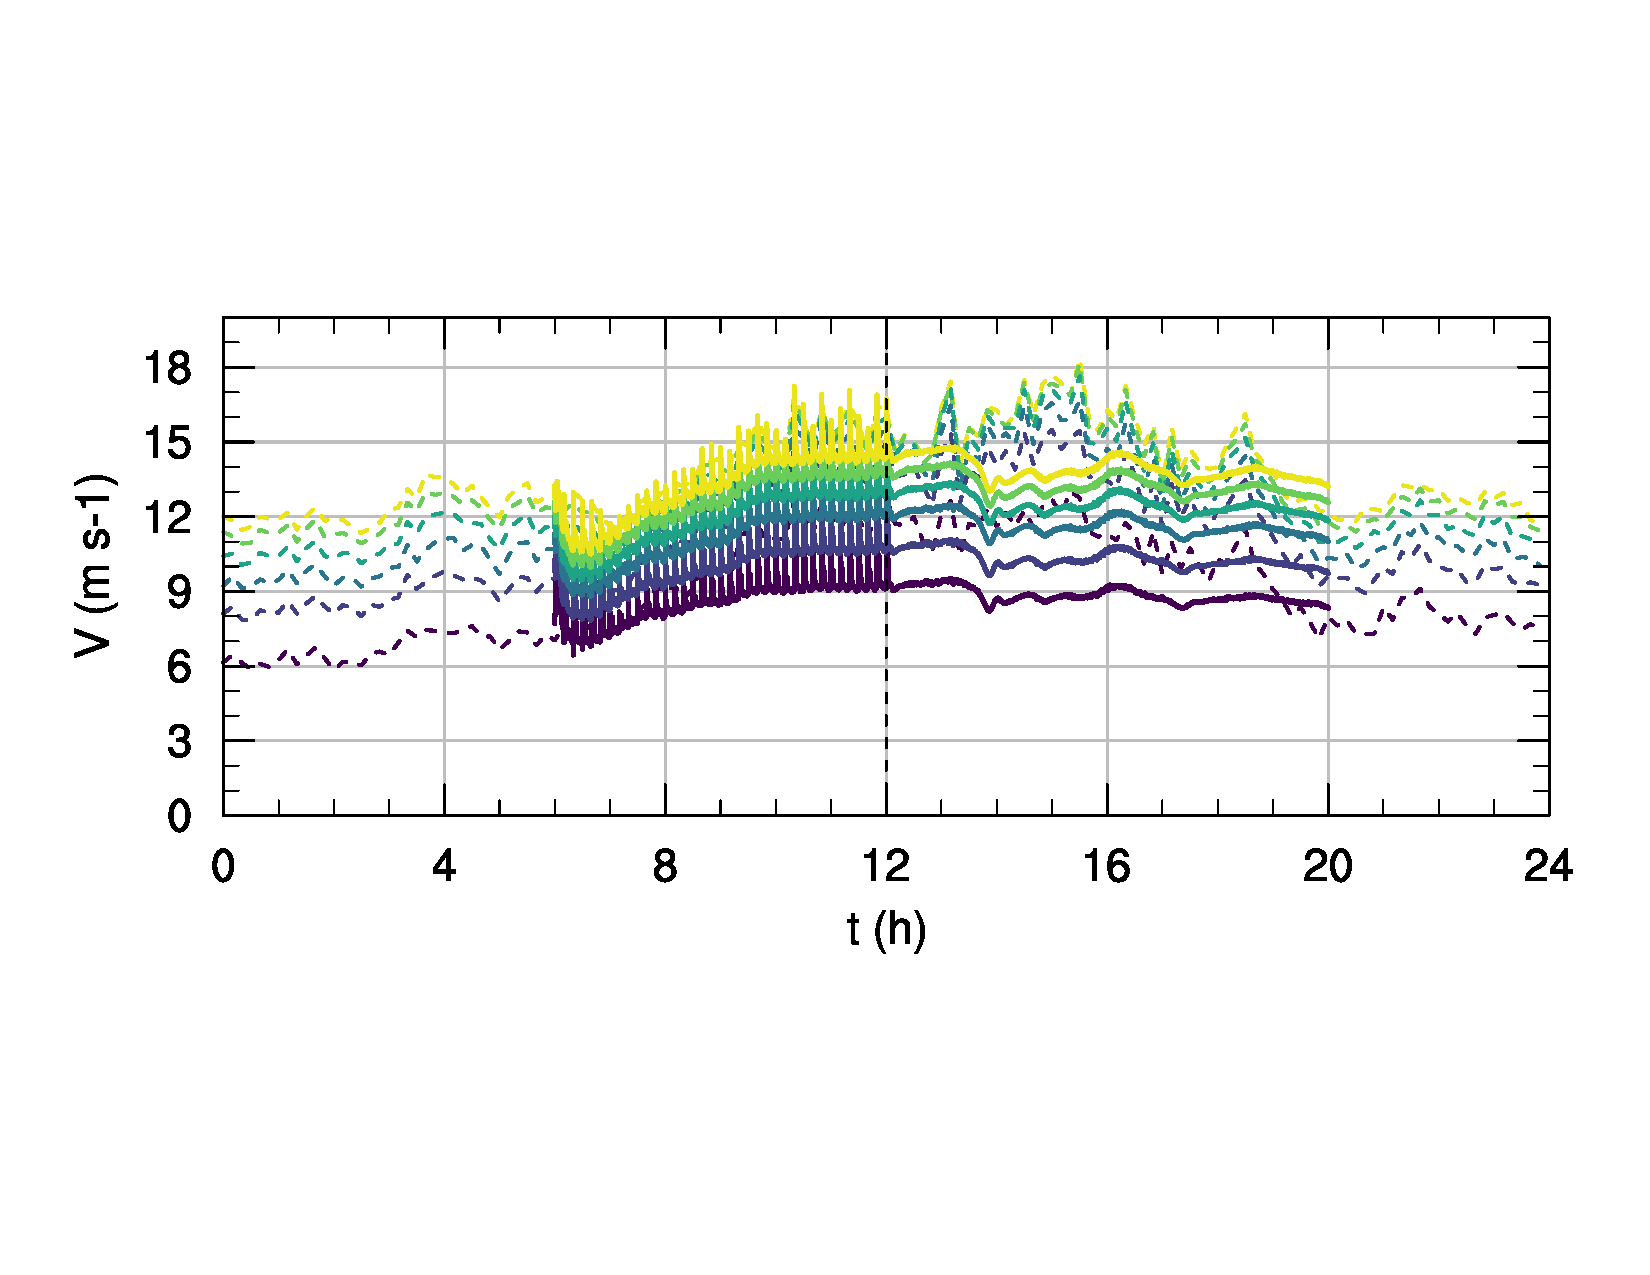
\includegraphics[width=0.5\linewidth,trim={9mm 63mm 10mm 55mm},clip]{Imagenes/06/hov_da/ts_v}%
	
	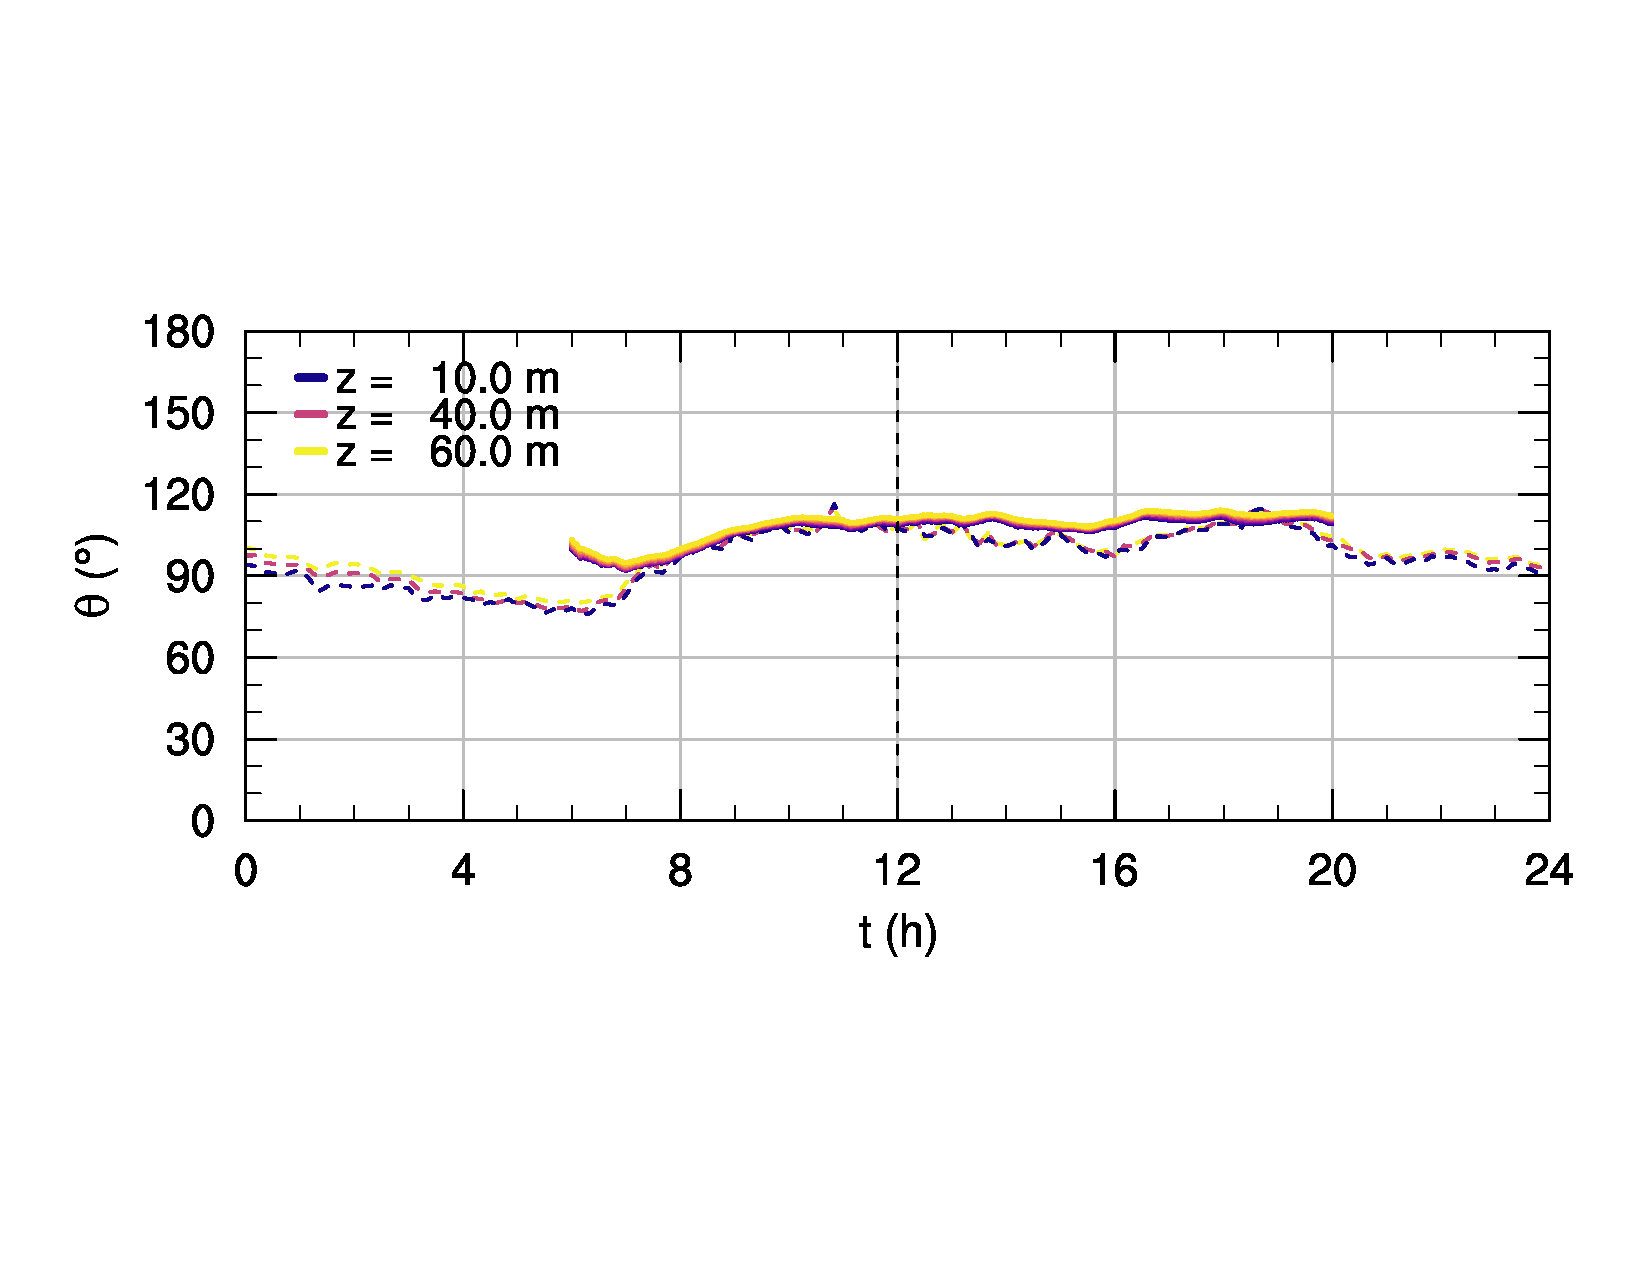
\includegraphics[width=0.5\linewidth,trim={12mm 55mm 10mm 55mm},clip]{Imagenes/06/hov/ts_o}%
	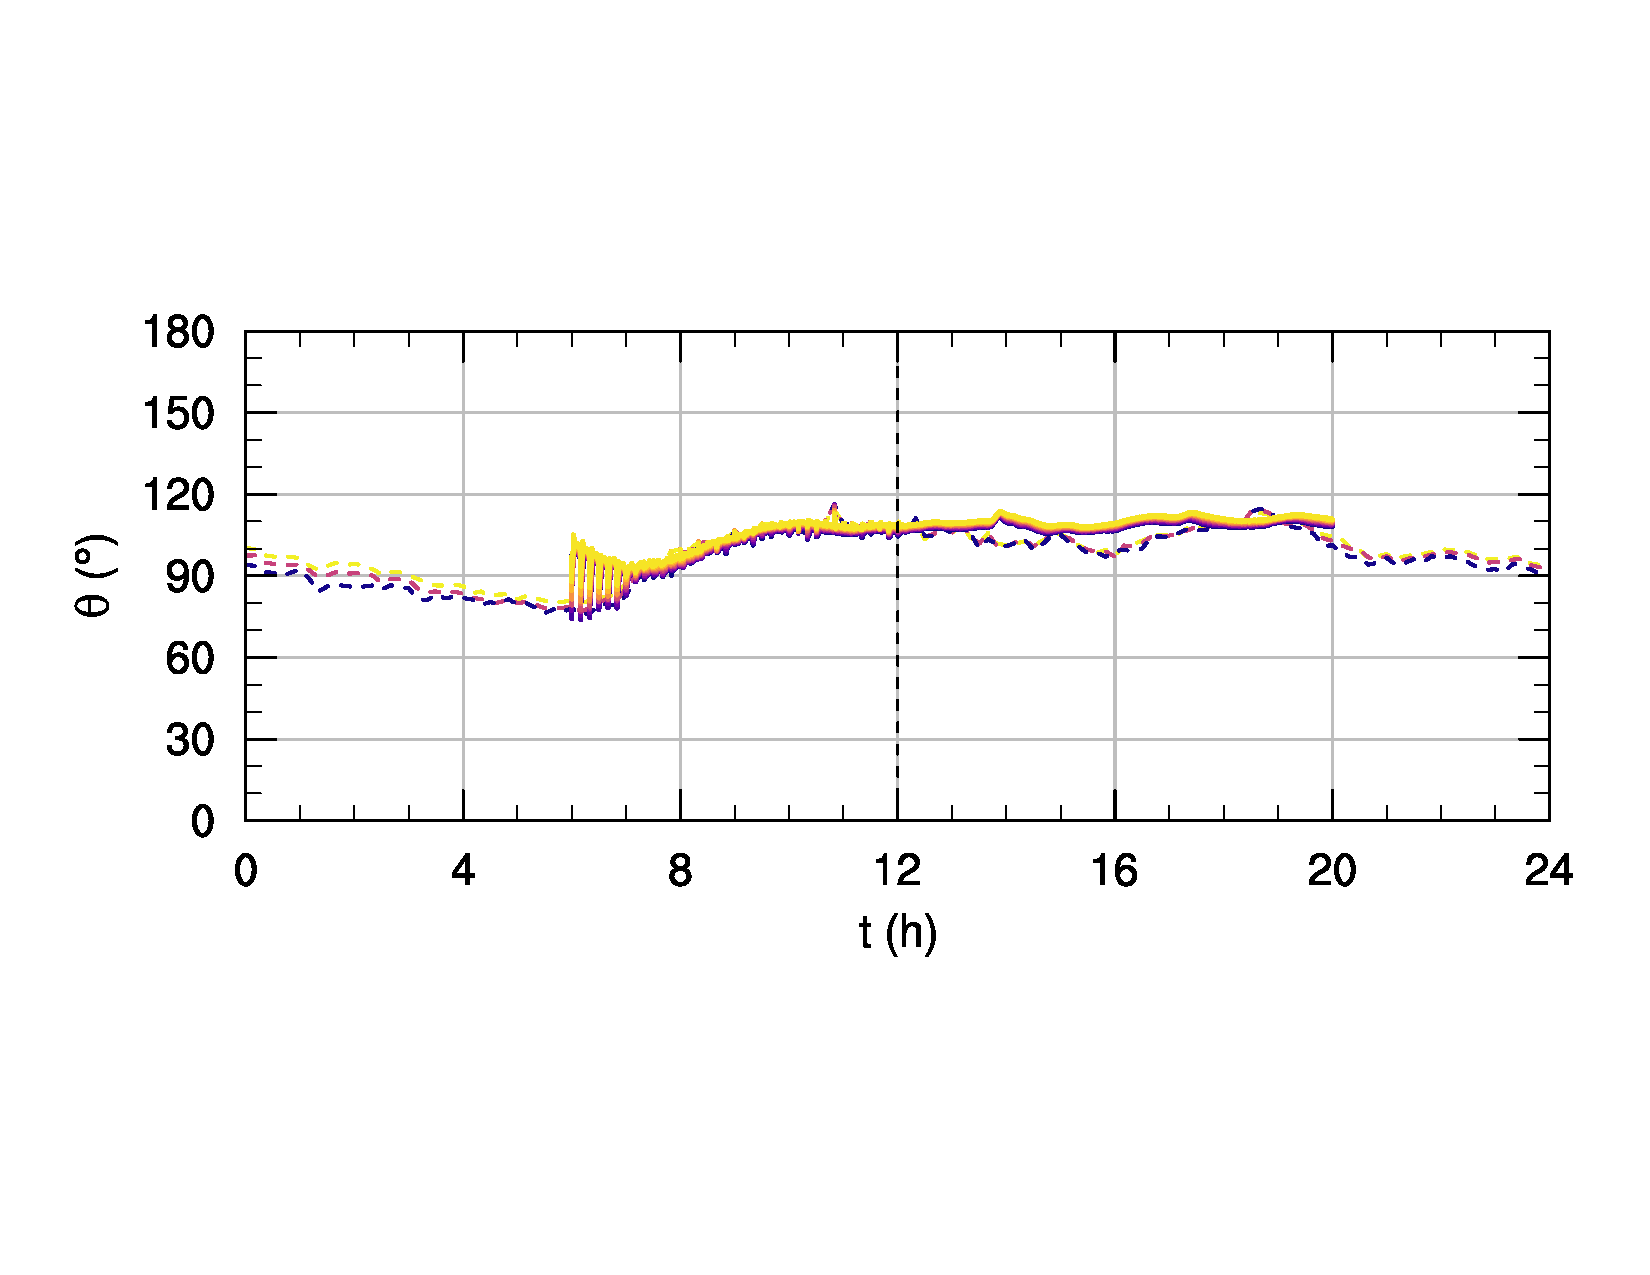
\includegraphics[width=0.5\linewidth,trim={12mm 55mm 10mm 55mm},clip]{Imagenes/06/hov_da/ts_o}%
	\caption{aaaaa}
	%\caption{Serie de tiempo para la rapidez instantánea del viento $V$ y su dirección en la ubicación del mástil meteorológico. La línea continua corresponde a lo datos simulados interpolados a las alturas de medición (solo para $V$) y la línea punteada a los datos medidos en el mástil.}
	\label{fig:06_hov_ts}
\end{figure}

\begin{figure}[H]
	\centering
	%\caption{Serie de tiempo para la rapidez instantánea del viento $V$ y su dirección en la ubicación del mástil meteorológico para el caso con asimilación de datos. La línea continua corresponde a lo datos simulados interpolados a las alturas de medición (solo para $V$) y la línea punteada a los datos medidos en el mástil.}
	\label{fig:06_hov_da_ts}
\end{figure}